\chapter{RSS Indoor localization}\label{sec:RSSIndoorLocalization}
This chapter describes most common techniques and methods for indoor localization using radio signal strength (RSS).

\section{Triangulation}\label{sec:Triangulation}
Methods based on Triangulation use geometric properties of triangles to determine target position. This can further be divided into Lateration and Angulation. \cite{RAinWILTaS} There are multiple sources of data these methods can use like distance estimation between device and specific transmitters, measurements of the signal propagation-time (TOA: Time Of Arrival and TDOA: Time Difference of Arrival\cite{LTinWSN}) and the direction of received
signal (AOA: Angle of Arrival\cite{AoALforWSN}).\cite{IILUBLEB}

\subsection{Lateration}\label{sec:Lateration}
Lateration refers to the technique of determining position based on distance measurements that are calculated using specific devices that know their own position.  Mainly used types of Lateration and are Trilateration and Multilateration. 

\begin{figure}[h!]
	\begin{centering}
		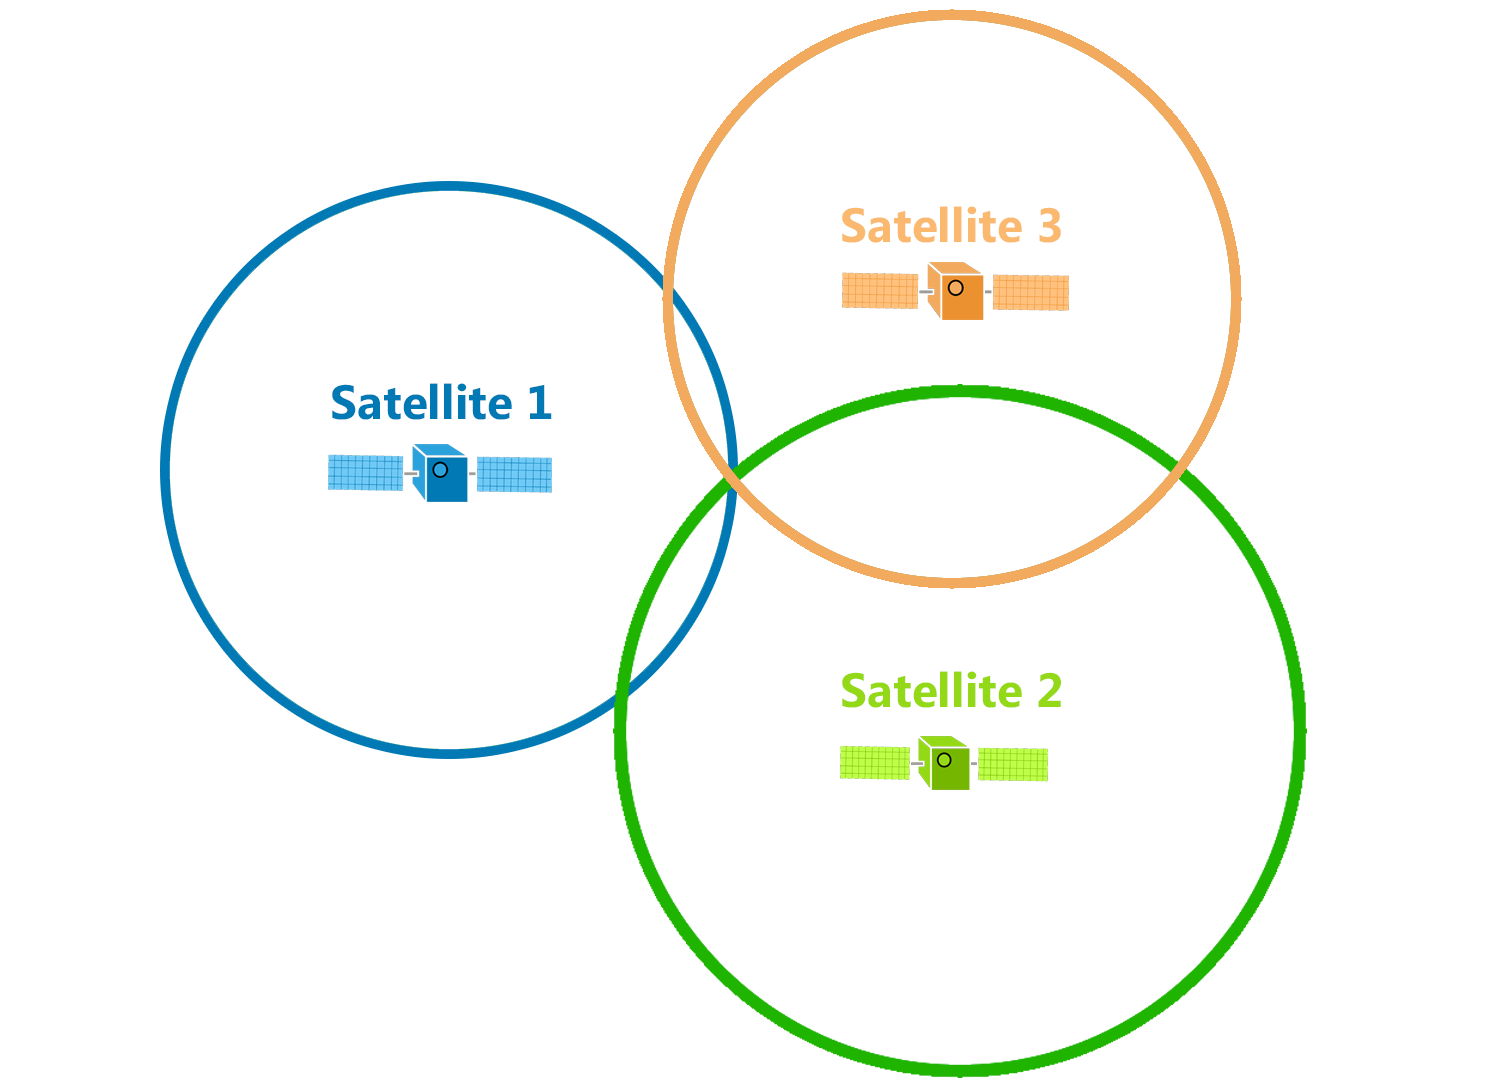
\includegraphics[width=0.48\textwidth]{img/trilateration_2d}
		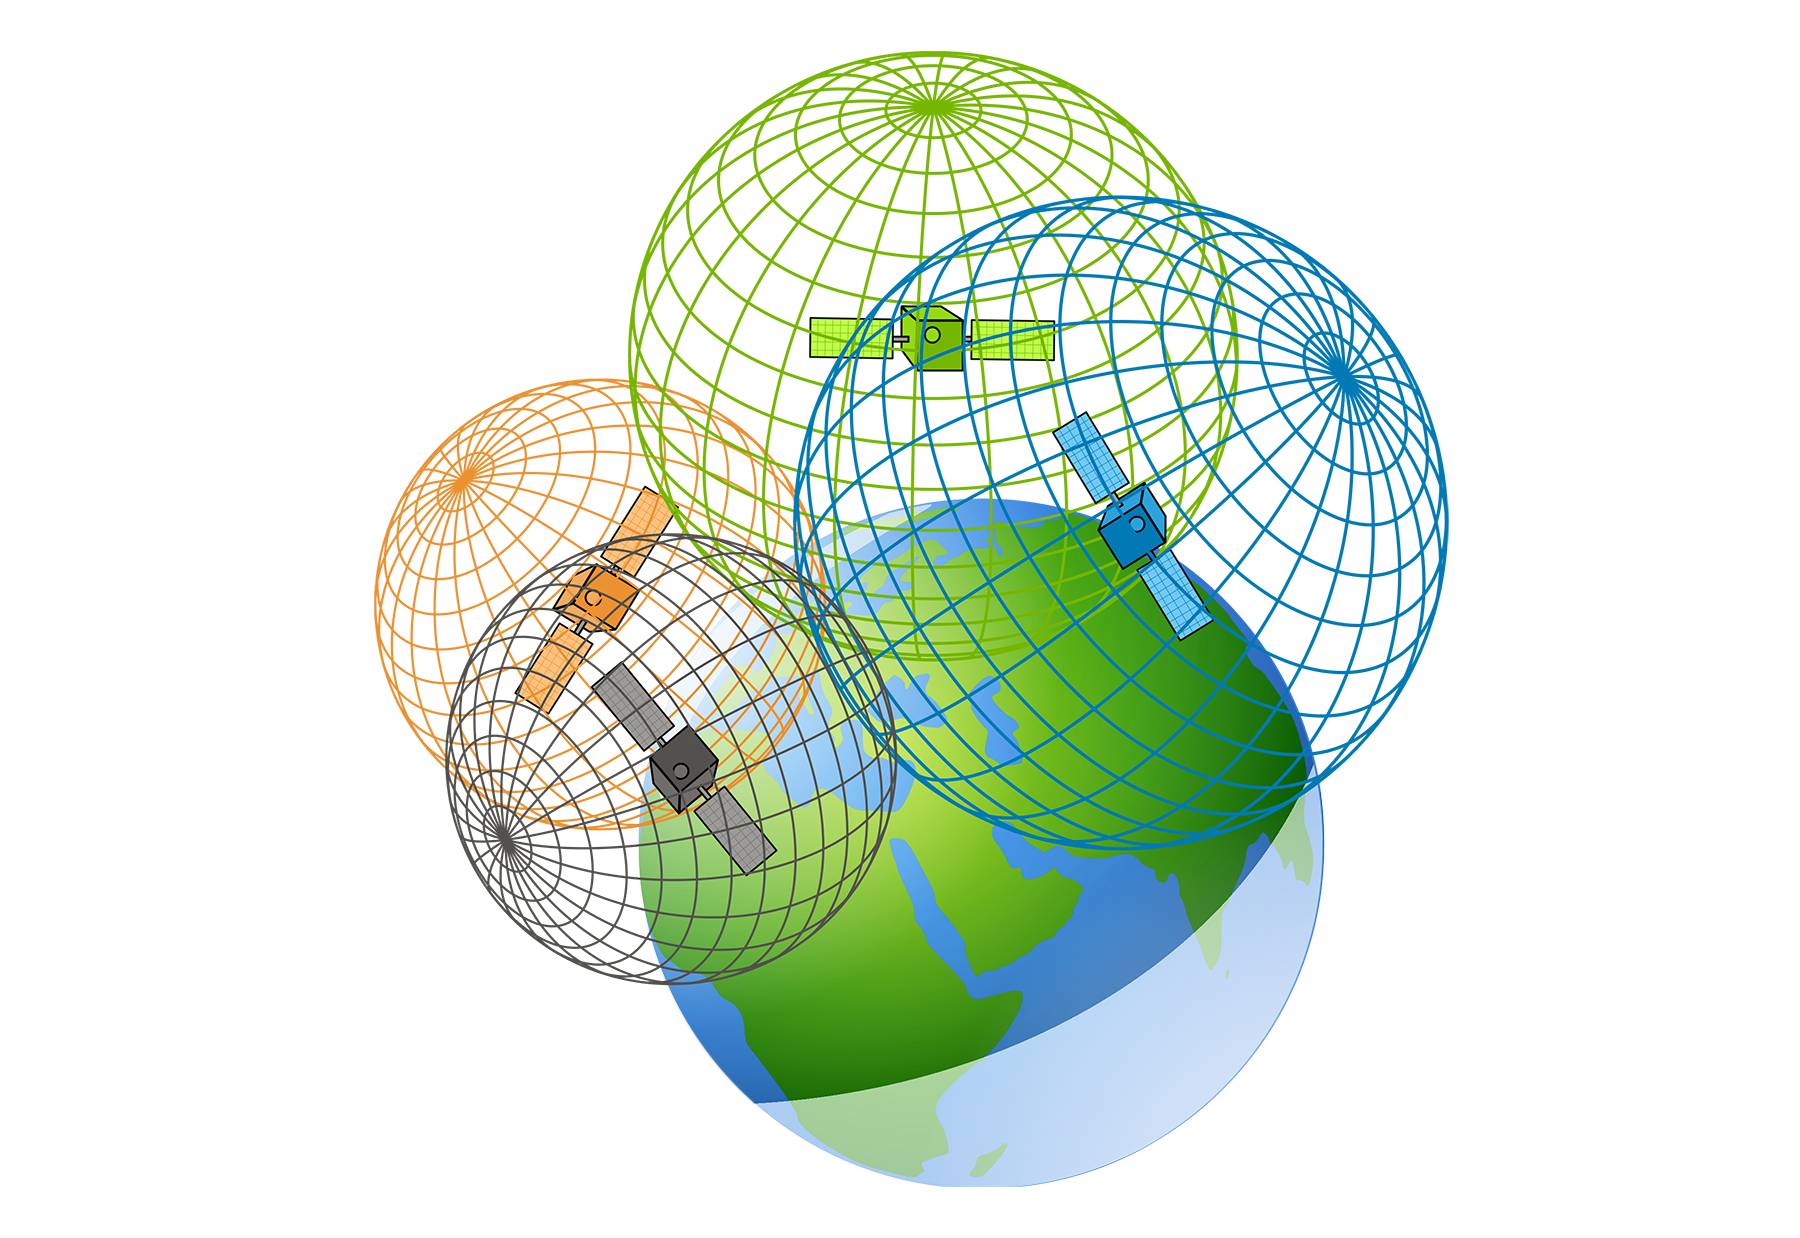
\includegraphics[width=0.48\textwidth]{img/trilateration_3d}
		\par\end{centering}
	\caption{2D and 3D Trilateration (source: \cite{TvTHGPSRW})\label{fig:2d_and_3d_trilateration}}
	\label{fig2}
\end{figure}

Trilateration uses distance measurements from at least three devices in particular as "tri" in the name suggests.\cite{RAinWILTaS} \fref{fig2} illustrates usage of Trilateration in 2D and 3D environment. While working in 2D plane will result with only one specific location point. Moving to the 3D plane can create a problem because signal is send in a sphere which could result in more than one position. That is the reason why some systems use at least four signal sources, example of such system is GPS.\cite{GNSSGPS} Advantage is easy implementation and simple calculations. One down side of this approach is that all devices must have synchronized clock.\cite{RAinWILTaS}

Multilateration also known as hyperbolic positioning is using Time Difference of Arrival (TDoA) instead of Time Of Arrival (ToA) used in previous case. This approach involves the intersections of hyperbolas rather than circles as shown in \fref{fig3}. Main advantage of this method is that only receiving devices must have synchronized clock instead of all.\cite{PLTaA} Multilateration was developed for tracking aircraft position and it is widely used.

\begin{figure}[h!]
	\begin{centering}
		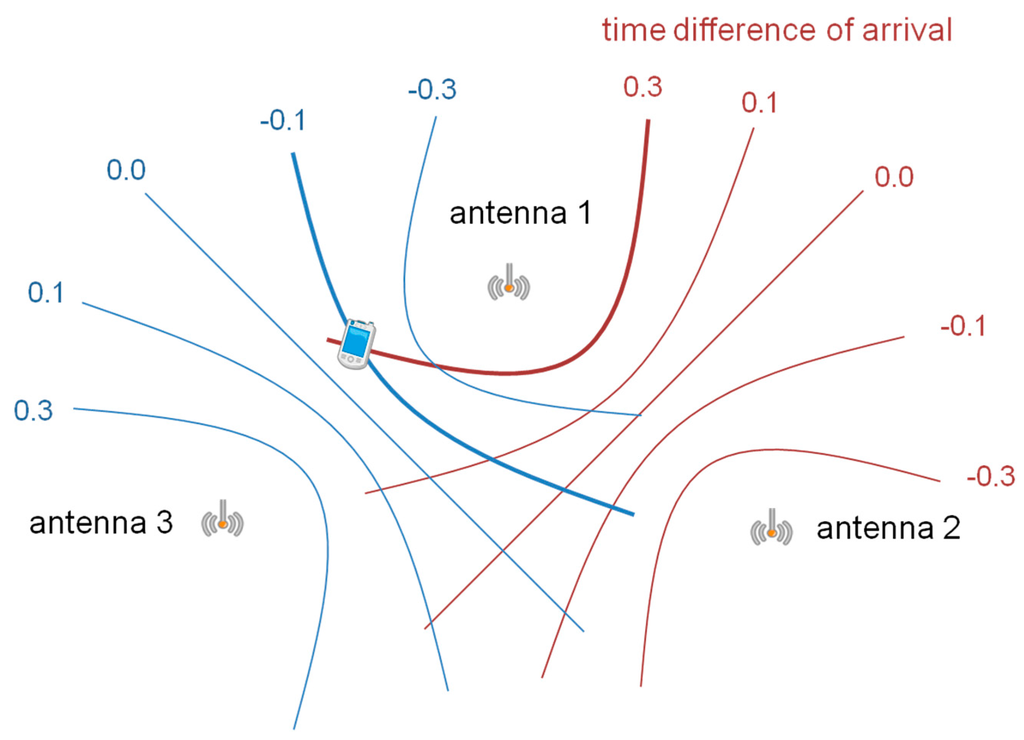
\includegraphics[width=0.6\textwidth]{img/multilateration}
		\par\end{centering}
	\caption{Multilateration (source: \cite{HPwAA})\label{fig:Multilateration}}
	\label{fig3}
\end{figure}

Note: At this time term Multilateration is not as strict as it used to be. It can now refer Lateration with more than three devices.

\subsection{Angulation}\label{sec:Angulation}
This technique uses Angle of Arrival (AoA) of radio signals to determine location. It uses highly directional antennas or antenna arrays. Same as Lateration these antennas are placed in known location and basic AoA requires at least two of them to determine position on 2D plane but more of them can be used to improve accuracy.\cite{RAinWILTaS} That makes it an advantage over Trilateration. Second advantage of this approach is no need for synchronization between devices.

There are few disadvantages of this approach since it needs complex hardware setup due to the use of antennas. Other problem is with multipath locations since it can cause signal reflection making it not useful for indoor localization. And final one to mention is the decrease of accuracy when mobile target moves further from the antennas.\cite{AoA}\cite{RofAoA}

\begin{figure}[h!]
	\begin{centering}
		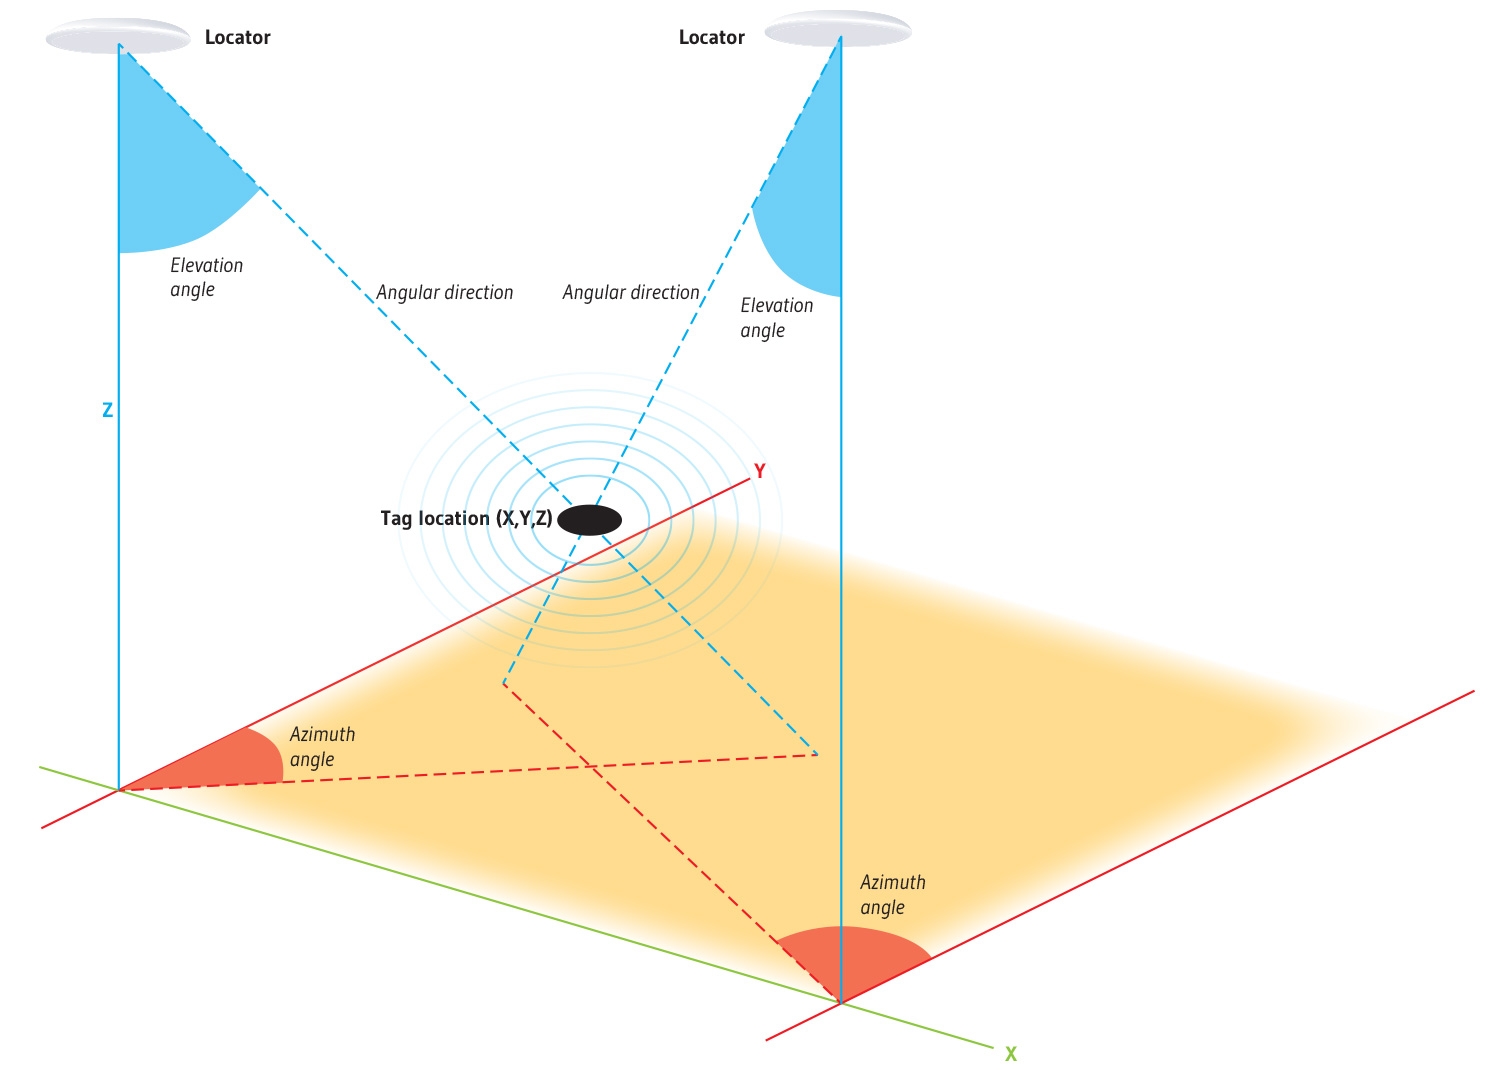
\includegraphics[width=0.6\textwidth]{img/angulation}
		\par\end{centering}
	\caption{3D location using AoA from Quuppa Intelligent Locating System (source: \cite{QAoA})\label{fig:AoAQuuppa}}
	\label{fig4}
\end{figure}

\section{Fingerprinting}\label{sec:Fingerprinting}
This method is a part of already mentioned Signal Strength Fingerprint Maps (SSFM) type. Main point of this method is using previously recorded data to figure out location inside the building. Hence fingerprint term in the name. There is multiple kinds of data that can be recorded like magnetic field strength or light signals but as it was already mentioned this topic is focused RSS. There are also multiple sources of radio signals like bluetooth, wireless or cellular devices and networks.

This method has two main stages where the first one is fingerprint maps construction also called offline stage. They are created using collecting Received Signal Strength (RSS) at different positions with specific coordinates of this place. All fingerprints are saved in the database and this is called fingerprint map. The other part is localization stage also known as online stage where client device measures data and compares them with fingerprint maps to approximate position. \cite{LocalizationApproaches}\cite{IndoorLocalizationWithoutThePain}

\section{Proximity}\label{sec:Proximity}
Proximity detection also knows as connectivity based positioning is one of the simplest method to implement.

\section{Other techniques}
%\section{Dead Reckoning}\label{sec:DeadReckoning}

%\section{K neighbors}\label{sec:KNeighbors}

%\section{Compressive sensing}\label{sec:CompressiveSensing}